% Talk 2 study paper: IEEE conference format (IEEEtran).
% Draft 1, 2026-10-04. Build: Overleaf (IEEEtran is built in), or `latexmk -pdf main.tex` / `tectonic main.tex`.
% Markers render in color and must all be gone before submission:
%   \pending{...}  a number from a run still in progress (round 3 follow-ups, 2026-10-04/05)
%   \verify{...}   a citation or external figure not yet checked against its source
%   \todo{...}     an open writing or design decision
% Every number traces to docs/TALK2-HARDWARE-SPECTRUM-TEST-LOG.md, docs/TALK2-DATA-ENGINEERING-IMPACT-TRACK.md
% or a script under deploy/aws-phone-proxies/scripts/; see README.md for the map.
\documentclass[conference]{IEEEtran}
\IEEEoverridecommandlockouts
\usepackage{cite}
\usepackage{amsmath,amssymb}
\usepackage{graphicx}
\usepackage{booktabs}
\usepackage{xcolor}
\usepackage{url}

\newcommand{\pending}[1]{\textcolor{orange}{[PENDING: #1]}}
\newcommand{\verify}[1]{\textcolor{red}{[verify: #1]}}
\newcommand{\todo}[1]{\textcolor{blue}{[TODO: #1]}}
\newcommand{\figplaceholder}[2]{\fbox{\parbox[c][#1][c]{0.92\columnwidth}{\centering\small #2}}}

\begin{document}

\title{Can the Phone in Your Pocket Take Work Off the Data Center?\\
Accuracy, Latency, and Energy of Small Language Models\\ Across the Consumer Hardware Spectrum}

\author{\IEEEauthorblockN{David Kjerrumgaard}
\IEEEauthorblockA{Datadog\\
dkjerrumgaard@gmail.com}}

\maketitle

\begin{abstract}
Large language model (LLM) inference is concentrating in data centers whose electricity and water demands are growing quickly. One proposed mitigation is to move narrow inference tasks onto consumer devices people already own. We test that proposition on a real, ground-truthed task, LLM triage of connected-vehicle telemetry, by running identical small language models (17 GGUF models of 0.34--9.4B parameters, one llama.cpp build) across a consumer hardware spectrum: cloud stand-ins for mainstream and flagship Android CPUs, Apple M1 and M4 systems (iPhone-class silicon), and an M4~Max laptop, with a Raspberry Pi~4 as a dedicated edge-board baseline. We measure task accuracy with confidence intervals clustered by test case, end-to-end latency and job completion, and energy above idle per decision. Phone-class silicon answers a triage call in 1--2\,s versus 32\,s on the Pi~4, at 7--10$\times$ less energy per call, and on a single chip the CPU spends 1.4--4$\times$ the energy per token of the GPU. A changed prompt costs the Pi~4 5$\times$ a repeated one, or 2.7$\times$ with the fixed instructions first. Accuracy is invariant across hardware but not across quantization format, task scope, prompt format, or reasoning mode: reasoning (``thinking'') adds no measurable accuracy at 4--11$\times$ the latency, and asking small models to perform the whole task rather than one bounded judgment drops accuracy from 94--100\% to 11--22\%. End to end, the edge design saves energy less through where the model runs than through filtering events before the model and not transmitting raw telemetry.
\end{abstract}

\begin{IEEEkeywords}
edge AI, small language models, energy efficiency, on-device inference, quantization, benchmarking, sustainable computing
\end{IEEEkeywords}

% =====================================================================
\section{Introduction}
% =====================================================================

AI adoption is driving rapid growth in data-center electricity demand, with corresponding water and carbon costs~\cite{iea2025energyai,luccioni2024power}. Data centers will remain necessary, but a share of inference requests are narrow, repetitive decisions that may not need a frontier model or a remote GPU at all. Consumer devices are a large pool of already-deployed compute: a current smartphone carries a multi-core CPU, a GPU, and a neural accelerator, and is powered on for most of the day. If even a small fraction of narrow inference work could run on such devices, the data-center share of that work would shrink.

Whether that is true depends on three empirical questions. Can a small model do a real task accurately enough? Is it fast enough on consumer hardware, and does it reliably finish? And does running it there actually use less energy, end to end? Benchmarks of on-device LLMs typically report tokens per second or joules per token on synthetic prompts~\cite{laskaridis2024melt}; they rarely tie those numbers to a scored task or follow the energy beyond the chip.

We study these questions on a concrete workload: an edge triage pipeline for connected trucks, in which an LLM running on the vehicle decides which ETA-threatening slowdowns are worth reporting to a control center over cellular. The task has an exact answer key, so every model output is scored automatically. We run the same models, prompts, decoding settings, and runtime across six platforms: stand-ins for mainstream and flagship phones, Apple systems up to a developer laptop, and a 2019 single-board computer as the baseline for a dedicated edge box, and we measure accuracy, latency, completion, and energy.

We address six research questions:
\begin{itemize}
\item \textbf{RQ1 (speed):} How fast do identical small models run across the consumer spectrum, and how close are the stand-ins to real phones?
\item \textbf{RQ2 (energy):} What does one decision cost in energy on each class of device, and on CPU versus GPU within one device?
\item \textbf{RQ3 (accuracy):} Does accuracy depend on the hardware or on the quantization format?
\item \textbf{RQ4 (task scope and inference mode):} Can small models take on the whole task, and do the chat format and reasoning (``thinking'') help?
\item \textbf{RQ5 (deployment factors):} How do sustained load, server defaults, and memory capacity change outcomes?
\item \textbf{RQ6 (system energy):} Where does an edge deployment actually save energy?
\end{itemize}

Our contributions are: (1) a cross-spectrum measurement on one runtime and one model set, with phone stand-ins chosen by core lineage and calibrated against published phone figures; (2) per-decision energy on a scored workload, on CPU and GPU, alongside a wall-metered single-board computer; (3) a set of negative and confounding findings that matter for practitioners, including a reasoning-mode runaway, a quantization format that silently breaks one model, and a server default that exhausts device memory; (4) a methodological observation that, at production temperature, repeated trials of the same test case are strongly correlated, so confidence intervals must be clustered by case; and (5) a fully reproducible artifact.

% =====================================================================
\section{Background and Related Work}
% =====================================================================

\textbf{On-device inference.} llama.cpp~\cite{llamacpp} runs quantized GGUF models on CPUs and GPUs (Metal on Apple silicon). Its 4-bit formats include the block-wise Q4\_0, the ``k-quant'' Q4\_K\_M with per-sub-block scales, and importance-weighted IQ4 variants; on ARM it repacks some formats at load time for faster kernels. Grammar-constrained decoding (GBNF) restricts generation to a formal grammar, which makes structured output reliable. Extremely low-bit models such as 1.58-bit BitNet~\cite{ma2024bitnet} motivated this study but were not usable on our ARM targets at the time (\S\ref{sec:threats}).

\textbf{Mobile LLM benchmarking and energy.} MELT~\cite{laskaridis2024melt} measured LLM inference on phones and edge boards, reporting throughput and energy per token \verify{MELT's headline energy figure}. Community benchmarks report per-model generation speed on recent iPhones~\cite{appleslmbench}, which we use for calibration. Token generation in LLMs is largely memory-bandwidth bound, so the Roofline model~\cite{williams2009roofline} and STREAM bandwidth~\cite{mccalpin1995stream} predict much of the speed ordering, though not all of it (\S\ref{sec:speed}).

\textbf{Energy of AI deployment.} Prior work quantified the energy and carbon of training~\cite{strubell2019energy,patterson2021carbon} and of inference across task types~\cite{luccioni2024power}. Providers have begun reporting per-prompt energy for production systems~\cite{elsworth2025google}. These studies concern data-center hardware; we measure consumer devices.

\textbf{Reasoning at test time.} Reasoning models trade extra generated tokens for accuracy; ``budget forcing'' caps the reasoning length by forcing the end-of-thinking delimiter~\cite{muennighoff2025s1}. We evaluate both uncapped and budget-forced reasoning on a short, bounded task.

\textbf{Offloading and radio energy.} Cellular radios spend substantial energy in promotion and tail states~\cite{huang2012lte}; modern low-power IoT modems change that balance~\cite{nepal2026ltem}. We use published radio measurements to place per-decision compute energy in a system context.

% =====================================================================
\section{Study Design}
% =====================================================================

\subsection{Workload and Ground Truth}

\textbf{The edge triage pipeline.} Each truck emits a telemetry event every 5\,s (532\,B of JSON: speed, position, planned versus current ETA, and derived signals such as ETA slip, stop-and-go index, peak deceleration, and ABS engagement). A deterministic gate forwards an event to the LLM only when a sustained slowdown coincides with an ETA slip of at least 3\,minutes. A deterministic classifier sets a baseline severity from the physics fields (ABS engaged forces high; deceleration and stop-and-go bands set the rest). The LLM receives the metrics plus context that thresholds cannot judge (weather, cargo, dispatch status) and writes, under a GBNF grammar, a one-paragraph risk synthesis and an escalation: \emph{raise}, \emph{hold}, or \emph{lower}. Final severity and the recommended action follow deterministically, and only cards with final severity \emph{high} are transmitted.

\textbf{Evaluations.} The \emph{Edge Triage} evaluation runs 60 calls per session: 15 for format reliability and 45 for escalation calibration (three scenarios, escalate-worthy, benign, and de-escalate-worthy, 15 calls each), scored against each scenario's documented expected direction. A second task, \emph{Tier~2}, has the model turn a correlated multi-truck slowdown into a two-to-three-sentence spoken warning, scored for grounding and speakability (30 calls).

\textbf{Round 3: task scope and inference mode.} To test whether newer hardware and larger models can take back the work that deterministic code took over, we define a \emph{full} task in which the model also classifies the baseline severity from stated physics rules and derives the final severity and action, all in one call. The deterministic code is the answer key. Cases span six physics profiles crossed with the three scenarios (18 cells, two repetitions each, 36 calls); the production \emph{narrow} task uses the canonical event and three scenarios (3 cells, six repetitions each, 18 calls). A call is correct end to end (\emph{all\_ok}) when its format, baseline, escalation, severity, and action are correct and internally consistent. We also vary how the prompt reaches the model: \emph{raw} completion (production), the model's chat format with reasoning off (\emph{chat-off}) or on (\emph{chat-on}, 2,048-token budget), and budget-forced reasoning (\emph{chat-budget}, 1,024 tokens). A prompt ablation adds seven cumulative variants (explicit physics facts, lookup tables, the native chat template, worked examples, temperature 0, and grammar-computed derived fields), fixed before any result was observed.

\subsection{Platforms and Proxy Fidelity}

Table~\ref{tab:platforms} lists the platforms. Real phones were out of scope for this round; instead we chose stand-ins by core lineage and calibrated them. Cloud ARM instances stand in for Android CPUs: Graviton3 (Neoverse V1), built without SVE and i8mm to match a Cortex-X1-class phone core, and Graviton5 (Neoverse V3) for a current flagship. Both have more memory bandwidth than the phones they represent (202 and 121\,GB/s, against about 85\,GB/s for a current flagship), so their speeds are upper bounds. An Apple M1 matches published iPhone~17~Pro generation speed within 9\% on the two calibration models (\S\ref{sec:speed}), so we treat it as the iPhone-class stand-in. The Raspberry Pi~4 is a real-device baseline for the alternative to a phone: a dedicated edge board, bought and powered for this task alone.

\begin{table}[t]
\caption{Platforms. Bandwidth is measured with STREAM where noted (m), otherwise the vendor figure (v).}
\label{tab:platforms}
\centering
\small
\begin{tabular}{@{}llll@{}}
\toprule
Platform & Stands in for & Mem. BW (GB/s) & Energy \\
\midrule
Raspberry Pi 4 (8\,GB) & dedicated edge board & \todo{} & wall meter \\
Graviton3 c7g, X1 build & mainstream Android & 202 (m) & -- \\
Graviton5 c9g & flagship Android & 121 (m) & -- \\
Apple M1 (16\,GB) & iPhone 17 Pro class & 68 (v) & chip \\
Apple M4 (24\,GB) & newer Apple silicon & 120 (v) & chip \\
Apple M4 Max (64\,GB) & developer laptop & \verify{546} (v) & chip \\
\bottomrule
\end{tabular}
\end{table}

\subsection{Models and Runtime}

All platforms run llama.cpp v0.5.0 (commit \texttt{7fe450e}), with Metal on Apple silicon and CPU elsewhere. Seventeen instruction-tuned GGUF models span 0.34--9.4B parameters (Granite~4.0 350M, LFM2.5 350M, Qwen2.5 0.5/1.5/3B, Qwen3 0.6/8B, Gemma~3 1/4B, Gemma~4 E2B, Llama~3.2 1/3B, Qwen3.5 2B, Phi-3.5-mini, Ling-3.0-tiny, Llama~3.1~8B, GLM-4-9B), all at Q4\_K\_M unless stated; round~3 adds Gemma~3/4 12B, Qwen3-14B, Qwen3.5-9B, and Qwen3.8-27B~\cite{abdin2024phi3,gemma2025gemma3,yang2025qwen3,grattafiori2024llama3,glm2024chatglm}. Every model file is pinned by repository revision and SHA-256 (105 files), and hashes were re-verified on every host after each run.

\subsection{Metrics}
\label{sec:metrics}

\textbf{Speed and completion.} We report llama-bench prompt processing (pp512) and generation (tg128) throughput, and for the real workload the per-call latency median (p50) and 95th percentile (p95). A call that hits its token budget or timeout counts as incomplete and incorrect.

\textbf{Energy.} On Apple silicon we sample combined CPU, GPU, and neural-engine power with \texttt{powermetrics} every 500\,ms, subtract an idle baseline from interleaved idle windows, and integrate over each session window. Energy per call is session energy divided by calls, an upper bound that includes server start-up. Per-token energy uses llama-bench's per-repetition windows. On the Raspberry Pi~4 an inline USB-C meter measures whole-board power at the wall (idle 3.40\,W, two 10-minute baselines within 0.1\%). The cloud instances expose no power counters, so we report time only. The real-workload sessions repeat each test event, so after the first call the server reuses the prompt it has cached; \S\ref{sec:stream} measures calls whose prompt changes.

\textbf{Accuracy and uncertainty.} We report rates with 95\% Wilson intervals~\cite{wilson1927}. Because repeated calls on the same case are correlated (\S\ref{sec:icc}), we compute each interval at an effective sample size $n_{\mathrm{eff}} = n / (1 + (m-1)\rho)$~\cite{kish1965}, where $m$ is the mean number of calls per case and $\rho$ is the within-case intraclass correlation of correctness, estimated per session by one-way ANOVA and clipped to $[0,1]$ (taken as 1 when outcomes do not vary at all, so $n_{\mathrm{eff}}$ equals the number of cases).

\subsection{Controls and Integrity}

Each model runs in its own server process and session; an early five-model session doubled one model's latency (\S\ref{sec:deploy}). On the laptop, every session waits for 60\,s of nominal thermal pressure, and runs are repeated in reverse order; the Mac mini hosts never left nominal thermal pressure (10,593 and 7,179 samples). Repeat runs on the M1 differ by a median of 0.1--0.2\%, and a reverse-order repetition of the real workload changed p50 by under 4\% and energy per call by under 2\%. After we found that the server's default context size reserves each model's full training context (\S\ref{sec:deploy}), later laptop runs fixed it at 8,192 tokens, and a dedicated check measured the earlier runs' exposure.

% =====================================================================
\section{Results}
% =====================================================================

\subsection{Speed Across the Spectrum (RQ1)}
\label{sec:speed}

Generation speed tracks memory bandwidth to first order. On the calibration models, the M1 generates at 39.7 and 35.4\,tok/s (Qwen3.5-2B, Gemma-4-E2B) against published iPhone~17~Pro figures of 39.1 and 38.8\,tok/s~\cite{appleslmbench}; the M4 overshoots the phone by 1.5--1.7$\times$ (67.3, 59.1\,tok/s) and the flagship-Android stand-in by 1.4--1.5$\times$ (58.1, 54.6\,tok/s). Bandwidth is not the whole story: the Graviton3 instance has the most bandwidth (202\,GB/s) yet generates slower than the Graviton5 (40.6 vs 58.1\,tok/s on Qwen3.5-2B) and scales almost linearly with threads, so its older cores, not memory, are the limit. A build restricted to a Cortex-X1's instruction set ran 3--12\% \emph{faster} than the native build on the same instance, so the restriction did not inflate the stand-in. Fig.~\ref{fig:speed} shows the full spectrum.

\begin{figure}[t]
\centering
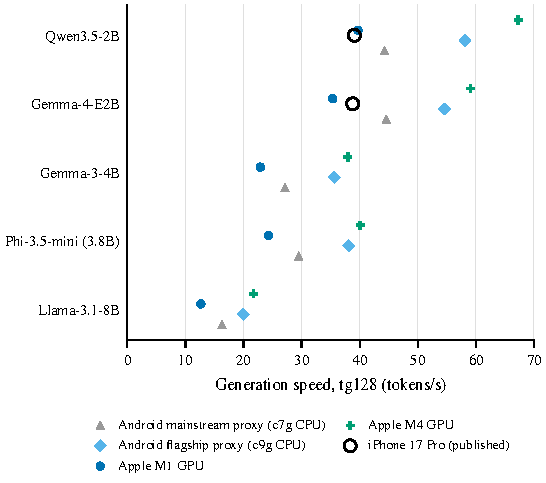
\includegraphics[width=\columnwidth]{figures/fig1_speed.pdf}
\caption{Generation throughput (tg128) of five representative models across the consumer spectrum, with published iPhone~17~Pro figures~\cite{appleslmbench}. Cloud stand-ins use 8 threads; Apple systems use the GPU (Metal). The Pi~4 ran only the real workload (Table~\ref{tab:realwork}).}
\label{fig:speed}
\end{figure}

On the real workload (Table~\ref{tab:realwork}), Phi-3.5-mini answers a triage call in 31.7\,s on the Pi~4, 1.9\,s on the M1, 1.2\,s on the M4, 1.1\,s on the flagship-Android CPU stand-in, and 0.36\,s on the laptop GPU. The CPU's disadvantage is largest in prompt processing, which is compute bound (Table~\ref{tab:cpugpu}).

\begin{table}[t]
\caption{Real workload: per-call latency (p50) and energy above idle per call, with each test event repeated, so the server reuses its cached prompt (calls whose prompt changes: Table~\ref{tab:stream}). Pi~4 energy is whole-board at the wall; Apple figures are chip-level.}
\label{tab:realwork}
\centering
\small
\begin{tabular}{@{}lrrrr@{}}
\toprule
 & \multicolumn{2}{c}{Phi-3.5, Edge Triage} & \multicolumn{2}{c}{Gemma-3-4B, Tier 2} \\
Platform & p50 (s) & J/call & p50 (s) & J/call \\
\midrule
Raspberry Pi 4 & 31.7 & 154 & 43.7 & 208 \\
Graviton5 (CPU) & 1.08 & -- & \todo{} & -- \\
Apple M1 (GPU) & 1.91 & 20.0 & 2.67 & 27.1 \\
Apple M4 (GPU) & 1.18 & 15.2 & 1.66 & 21.5 \\
Apple M4 Max (GPU) & 0.36 & $\sim$15 & 0.50 & $\sim$23 \\
\bottomrule
\end{tabular}
\end{table}

\subsection{Energy per Decision (RQ2)}
\label{sec:energy}

Across device classes, the Pi~4 spends about 154\,J above idle per triage call when the prompt repeats (288\,J including idle), while iPhone-class and newer Apple GPUs spend 15--20\,J at chip level (Table~\ref{tab:realwork}). The boundary differs (wall versus chip), but doubling the Apple figures to allow for power delivery and memory still leaves the Pi several times higher. The reason is time: the Pi draws about 7.3\,W during inference versus 3.4\,W idle, but takes 17--90$\times$ longer per call.

Within one chip, the comparison is like for like. Table~\ref{tab:cpugpu} shows energy per token on the M1's CPU and GPU for the same model files. The CPU spends about 4$\times$ the energy per token in prompt processing and 1.4--1.6$\times$ in generation for 3--9B models; only the smallest models (under 1B) generate at similar or lower energy on the CPU. Both phases cost more on the CPU, so a decision does too. On the GPU, by contrast, a generated token costs about 9$\times$ the energy of a prompt token (Phi-3.5: 421 vs 49\,mJ), so per-call energy follows answer length more than prompt length (\S\ref{sec:round3}). Fig.~\ref{fig:energy} shows both comparisons.

\begin{figure}[t]
\centering
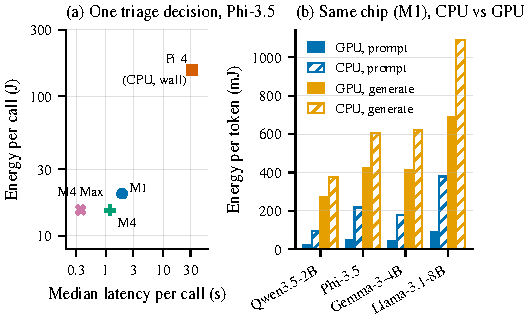
\includegraphics[width=\columnwidth]{figures/fig2_energy.pdf}
\caption{(a) Median latency and energy above idle for one Edge Triage decision (Phi-3.5-mini); the Pi~4 is metered at the wall, the Apple systems at the chip. (b) Energy above idle per token on the same Apple M1, GPU versus CPU (4 threads), for prompt processing and generation.}
\label{fig:energy}
\end{figure}

\begin{table}[t]
\caption{Apple M1, same model files: energy above idle per token (mJ) on GPU (Metal) and CPU (4 threads).}
\label{tab:cpugpu}
\centering
\small
\begin{tabular}{@{}lrrrr@{}}
\toprule
 & \multicolumn{2}{c}{Prompt (pp512)} & \multicolumn{2}{c}{Generation (tg128)} \\
Model & GPU & CPU & GPU & CPU \\
\midrule
Qwen3.5-2B & 19 & 93 & 272 & 375 \\
Phi-3.5-mini (3.8B) & 49 & 218 & 421 & 604 \\
Gemma-3-4B & 42 & 178 & 412 & 622 \\
Llama-3.1-8B & 89 & 379 & 689 & 1089 \\
\bottomrule
\end{tabular}
\end{table}

\textbf{When the prompt changes.}\label{sec:stream} A server's KV cache reuses a prompt only up to the first token that differs from the previous call's. The triage prompt carries the baseline severity and the trip context (weather, cargo, dispatch), not the per-event sensor readings, so consecutive calls about one truck in one incident usually repeat it, which is what Table~\ref{tab:realwork} measures: the server read 1 of 514 prompt tokens per call. The prompt changes with the first call of an incident, a changed context field or baseline, a once-per-incident policy, or a device that triages several trucks. The production prompt places the event's fields before the decision rules, so a changed event re-reads about 400 of its 514 tokens; moving the fields after the rules, with the wording otherwise unchanged, cuts this to about 148, at unchanged accuracy on llama-server (100\% format, 0\% escalation mismatch over 45 calls). Through llama-cpp-python, with the same model file and sampling settings, the reordered prompt tipped the benign case from hold to lower on every call (15 of 45 escalations mismatched on the M4~Max CPU, 3 of 9 on the Pi~4), while the production order stayed correct (0 of 45); in-process, the Pi's changed calls cost the same as through llama-server (429\,J, 87\,s). Table~\ref{tab:stream} measures both on two devices, with the same servers and builds as Table~\ref{tab:realwork} and a different event on every call. On the laptop GPU a changed prompt costs 65\% more energy than a repeated one with the production prompt and 22\% more with the fields last. On the Pi~4 a changed call with the production order costs 772\,J and 160\,s, 5$\times$ a repeated one: reading 400 prompt tokens takes 129\,s, four times as long as generating the 42-token answer (31\,s). The reordered prompt halves this, to 416\,J and 82\,s (2.7$\times$ a repeated call), of which reading 148 tokens still takes 50\,s. Prompt order is a small lever on a GPU, where generation dominates, and a large one on a CPU, where reading the prompt does.

\begin{table}[t]
\caption{Phi-3.5-mini, Edge Triage: a repeated prompt (Table~\ref{tab:realwork}) versus a different event on every call, for two orders of the same prompt. Prompt tokens read per call of 514 (median). Pi~4: 18 calls per row, whole board at the wall. M4 Max: 2--3 sessions of 60 calls, chip level. Changed calls with the production order ran with one server slot and no host-memory prompt cache, so recurring test events cannot be restored from an earlier copy.}
\label{tab:stream}
\centering
\small
\begin{tabular}{@{}lrrrrr@{}}
\toprule
 & & \multicolumn{2}{c}{Raspberry Pi 4} & \multicolumn{2}{c}{M4 Max (GPU)} \\
Calls & Read & p50 (s) & J/call & p50 (s) & J/call \\
\midrule
Repeated & 1 & 31.7 & 154 & 0.36 & $\sim$15 \\
Changed, as built & 400 & 160 & 772 & 0.70 & 25.0 \\
Changed, fields last & 148 & 82.2 & 416 & 0.49 & 18.5 \\
\bottomrule
\end{tabular}
\end{table}

\subsection{Accuracy Across Hardware and Quantization (RQ3)}
\label{sec:accuracy}

\textbf{Hardware.} Accuracy did not depend on the hardware. On round~3, the M1 and the M4~Max agree on every one of the 28 model-task-mode cells within their clustered intervals, and in 83\% of full-task cases every call on both machines was scored the same (all correct or all incorrect). Earlier, the Pi~4 matched the laptop within 6 percentage points on three models. Model file, runtime, and decoding settings determine answers; the hardware determines speed. The runtime matters on its own: through llama-cpp-python instead of llama-server, with the same model file and sampling settings, Phi-3.5 moved two borderline escalations from hold to lower on every call, on the M4~Max CPU and on the Pi~4 alike (\S\ref{sec:stream}).

\textbf{Quantization.} The format did matter (Table~\ref{tab:quant}). Replacing Q4\_K\_M with Q4\_0 reduced energy per call by 14--41\% on the M1 and 10--36\% on the M4 and sped up ARM CPU generation 1.4--1.7$\times$, but it raised Gemma-3-4B's escalation mismatch from 0\% to 30.4\% and doubled Llama-3.1-8B's, while the other models held. The importance-weighted IQ4 formats also degraded Gemma-3-4B.

\begin{table}[t]
\caption{Escalation mismatch by 4-bit format (Edge Triage, 270 escalation calls per format; M4).}
\label{tab:quant}
\centering
\small
\begin{tabular}{@{}lrrrr@{}}
\toprule
Model & Q4\_K\_M & Q4\_0 & IQ4\_XS & IQ4\_NL \\
\midrule
Gemma-3-4B & 0.0\% & 30.4\% & 23.3\% & 16.7\% \\
Llama-3.1-8B & 6.3\% & 14.4\% & -- & -- \\
\bottomrule
\end{tabular}
\end{table}

\subsection{Task Scope and Inference Mode (RQ4)}
\label{sec:round3}

Table~\ref{tab:round3} summarizes round~3 on the laptop (the M1 replicates every cell within its interval).

\begin{table}[t]
\caption{Round 3, end-to-end correctness (\%) with 95\% intervals clustered by case. Narrow: 3 cases $\times$ 6; full: 18 cases $\times$ 2 (Qwen3.8-27B: $\times$1). M4~Max.}
\label{tab:round3}
\centering
\footnotesize
\setlength{\tabcolsep}{3pt}
\begin{tabular}{@{}lllll@{}}
\toprule
Model & Narrow, raw & Full, raw & Full, chat-off & Full, chat-on \\
\midrule
Phi-3.5-mini & 100 [44--100] & 11 [4--29] & & \\
Gemma-3-4B & 100 [44--100] & 22 [9--45] & & \\
Llama-3.1-8B & 94 [74--99] & 14 [5--35] & & \\
GLM-4-9B & 89 [56--98] & 39 [20--61] & & \\
Gemma-3-12B & 72 [27--95] & 58 [37--77] & & \\
Gemma-4-12B & 67 [26--92] & 50 [30--70] & & \\
Qwen3-8B & 100 [44--100] & 36 [19--58] & 44 [25--66] & 47 [28--67] \\
Qwen3-14B & 33 [6--79] & 42 [24--62] & 72 [49--88] & 78 [59--90] \\
Qwen3.5-9B & 56 [21--86] & 22 [10--43] & 72 [51--87] & 0 [0--18]$^\dagger$ \\
Qwen3.8-27B & 78 [45--94] & 33 [16--56] & 67 [44--84] & 67 [44--84] \\
\bottomrule
\multicolumn{5}{@{}l}{$^\dagger$All 36 calls exhausted the reasoning budget.}
\end{tabular}
\end{table}

\textbf{Task scope.} Small models handle one bounded judgment but not the whole task. Phi-3.5-mini, Gemma-3-4B, and Llama-3.1-8B score 94--100\% on the narrow task and 11--22\% on the full task. Every component degrades: baseline severity 53--78\% correct, internal consistency 47--53\%, and even the escalation 53--58\%. In production's prompt mode no model exceeds 58\% on the full task, even at 12--27B parameters.

\textbf{Prompt format.} Presenting the identical prompt in the model's own chat format with reasoning off raised Qwen3.5-9B from 22\% to 72\% on the full task (19\% to 61\% on the M1), with intervals well separated, at no extra compute. Qwen3-14B moved from 42\% to 72\% (33\% to 72\% on the M1), with overlapping intervals.

\textbf{Reasoning.} Turning reasoning on produced no measurable accuracy gain: 72$\to$78\% (Qwen3-14B), 44$\to$47\% (Qwen3-8B), and 67$\to$67\% (Qwen3.8-27B), all within each other's intervals, at 4--11$\times$ the median latency and, on the M1, 4--7$\times$ the energy per call (Qwen3-14B 202$\to$817\,J; Qwen3-8B 74$\to$540\,J). Qwen3.5-9B's reasoning did not terminate on the full task: at a 2,048-token budget all 36 calls were truncated, and at 4,096 tokens 35 of 36 still were (0\% correct, 128\,s per call). On the narrow task, a 4,096-token budget left only 2 of 18 truncated (61\% [20--91]), so there the 2,048-token budget was simply too tight. Fig.~\ref{fig:thinking} shows the trade-off: reasoning moves every model to the right without moving it up. Budget forcing at 1,024 tokens fixed completion without improving accuracy. On all three Apple machines no call was truncated: Qwen3.5-9B reached the cap on every call and still answered. Every capped result lay within the interval of reasoning off (e.g.\ Qwen3-14B, full task: 72\% off, 72--83\% capped; Qwen3.5-9B: 61--72\% off, 64--67\% capped). It cost 3--10$\times$ the energy and 3.5--17$\times$ the median latency per call. On the M1, Qwen3-14B's full-task call rose from 202 to 768\,J, and Qwen3.5-9B's narrow-task call from 99 to 960\,J (105\,s). \textbf{Prompt engineering.} The prompt ablation (seven cumulative variants fixed in advance; the M4~Max and M4 agree within their intervals) shows prompt structure matters as much as model size.
\begin{itemize}
\item Physics facts, lookup tables, and the native chat template together raised Phi-3.5 from 11\% to about 50\%, Llama-3.1-8B from about 15\% to about 55\%, and Qwen3-14B from about 35\% to about 75\%.
\item Worked examples added 8--14 points, for Gemma-3-4B only. Temperature~0 and grammar-computed derived fields added nothing measurable.
\item On the M1, the template variant cost 9--52\% more energy per call than the base prompt, partly because answers grew longer.
\item Worked examples nearly doubled the prompt ($\sim$780 to $\sim$1,400 tokens) yet cost $-$12\% to $+$7\% energy, because answers got shorter (Phi-3.5: 258 to 186 tokens).
\end{itemize}

\begin{figure}[t]
\centering
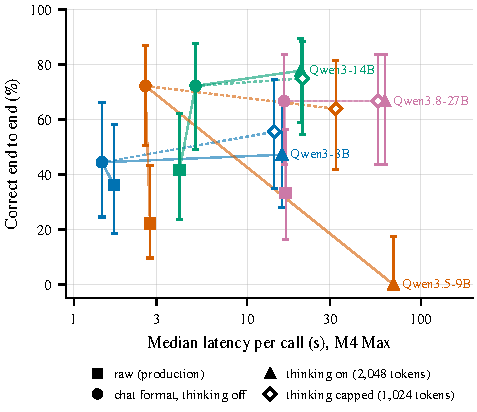
\includegraphics[width=\columnwidth]{figures/fig3_thinking.pdf}
\caption{Round 3, full task, M4~Max: end-to-end correctness (95\% intervals clustered by case) against median latency for four Qwen models in three prompt modes. Thinking adds latency without a measurable accuracy gain. Uncapped, Qwen3.5-9B's reasoning does not terminate within its budget; capped at 1,024 tokens (hollow diamonds, dashed from thinking off), every model answers, at no better accuracy than thinking off.}
\label{fig:thinking}
\end{figure}

\textbf{Repeated trials are correlated.}
\label{sec:icc}
At temperature 0.2, generated wording varied from call to call, but correctness was largely a property of the case: all repetitions of a case agreed in 90--92\% of full-task cases and 73--79\% of narrow-task cases, with a median intraclass correlation of 0.8. Treating calls as independent would overstate precision; for example, 18 of 18 correct on the narrow task (3 cases) yields a clustered interval of [44, 100]\% rather than [82, 100]\%. Additional repetitions or additional machines add little information; additional distinct cases do.

\subsection{Deployment Factors (RQ5)}
\label{sec:deploy}

\textbf{Sustained load.} The laptop reached heavy thermal pressure within about 12 minutes of sustained inference. Thermally gated, cool sessions were 24--77\% faster than throttled ones but used 30--60\% more energy per call: throttling lowers clocks and power more than it lengthens each call. Without a fan, the Pi~4 throttled to 600\,MHz at 83.7\,$^\circ$C, and calls made in that state ran into the 300\,s timeout; fitting a fan removed the hard throttling. Both Mac mini hosts remained thermally nominal throughout.

\textbf{Server defaults.} With no context size configured, llama-server reserves each model's full training context (128k tokens for Phi-3.5 and Llama-3.1). On a 16\,GiB CPU host this exhausted memory and the server was killed; on the 64\,GB laptop it reserved about 50\,GB. A check at an 8,192-token context reduced resident memory to about 6\,GB with no measurable change in latency or energy per call for these models (Phi-3.5 p50 0.36--0.37\,s versus 0.37--0.38\,s; Llama-3.1 within its repetition spread), and on round~3's own task Phi-3.5's p50 was 2.81\,s versus 3.00\,s with identical accuracy. The ablation's base variant, round~3's full prompt at 8k, repeats the check for larger models on the laptop. Median latency stayed within the laptop's thermal variation of round~3's default-context runs (Gemma-3-4B 1.32 vs 1.37\,s, Llama-3.1-8B 2.16 vs 1.82\,s, Qwen3-14B 3.96 vs 4.06\,s), and accuracy stayed within interval. Qwen3.8-27B was not re-checked.

\textbf{Session structure.} Loading several models in one benchmark session doubled Phi-3.5's median latency (0.70 versus 0.36\,s) relative to a single-model session; results from multi-model sessions are not valid per-model latencies.

\textbf{Memory capacity.} Under cgroup memory caps at a small context, models up to 4B parameters fit in 4\,GiB, 8--9B models need 6\,GiB, 12B models 8\,GiB, and 14B models 12\,GiB. These are ceilings, not per-app phone budgets.

\subsection{Where the Energy Goes (RQ6)}
\label{sec:system}

\textbf{Filtering.} In 2.3 truck-days of simulated normal driving, the deterministic gate forwarded no events, so the LLM was never called. During an incident, the current pipeline calls the LLM on every 5\,s event, about 23 near-identical calls per incident (about 3.5\,kJ on the Pi~4); calling once per incident would cut this roughly 20$\times$.

\textbf{Transmission.} Streaming raw telemetry costs 9.2\,MB per truck per day; the edge pipeline transmits about 4\,KB per escalating incident and nothing on a normal day, about 2,300$\times$ less data. The energy saved depends on the radio: a 2012-era LTE smartphone radio streaming every 5\,s never leaves its connected tail state (about 1.06\,W, 92\,kJ per day)~\cite{huang2012lte}, so not transmitting dominates; a modern LTE-M modem streams the same data for about 2.5\,kJ per day~\cite{nepal2026ltem}, less than the edge compute on a Pi~4. Data-center ingestion and processing of the stream would add to the cloud side but were not measured.

\textbf{Calls times joules.} Fig.~\ref{fig:perday} combines the two factors. Without the gate, even the most efficient device would spend more energy on the LLM per day than an old LTE radio spends streaming everything; with the gate, the GPU devices fall well below the streaming cost of a modern IoT modem and the Pi~4 sits just above it, and calling once per incident lowers every bar by another factor of about 20, below even the modem. The choice of device moves each bar by about one order of magnitude; the invocation policy moves it by three to four. The bars use the repeated-prompt energy per call (Table~\ref{tab:realwork}). That fits the gated policy, whose calls within an incident mostly repeat the prompt, but not the once-per-incident policy, whose single call meets a changed prompt: on the Pi~4 it costs 5$\times$ more with the production prompt (2.7$\times$ with the fields last; \S\ref{sec:stream}), which leaves that bar still about 5$\times$ below the gated one.

\begin{figure}[t]
\centering
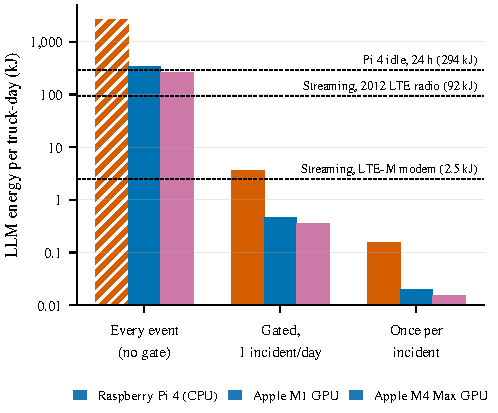
\includegraphics[width=\columnwidth]{figures/fig4_energy_per_day.pdf}
\caption{LLM energy per truck-day: calls per day $\times$ energy per call, for three invocation policies and three devices (one incident per day, 23 calls per incident). Dashed lines: the Pi~4's idle energy and the radio energy of streaming raw telemetry~\cite{huang2012lte,nepal2026ltem}. The hatched bar is infeasible in real time: the Pi~4 needs 31.7\,s per call against an event every 5\,s. Energy per call is the repeated-prompt figure; a changed prompt costs more (Table~\ref{tab:stream}).}
\label{fig:perday}
\end{figure}

\textbf{Idle.} The Pi~4's 3.4\,W idle (294\,kJ per day) exceeds every other term. A dedicated edge computer competes on energy only when it is a device that is powered on anyway, such as a phone or a vehicle's own computer, so that inference adds only marginal energy.

% =====================================================================
\section{Discussion}
\label{sec:discussion}
% =====================================================================

\textbf{Does moving inference to consumer devices reduce AI's footprint?} Not by itself, and not on CPUs. A slow CPU spends more energy per decision than a faster accelerator, both across devices and within one chip, because energy is power multiplied by time, and the CPU is slower both at reading the prompt and at generating the answer. The case for the edge rests instead on three things: (i) the accelerator already present in phone-class devices, which completed a triage decision for 15--20\,J at chip level; (ii) using hardware that is already powered on, so that only marginal energy counts; and (iii) the system architecture around the model, which avoided both the LLM call and the transmission for nearly all events.

\textbf{Theoretical arithmetic savings versus system energy.} Ternary (1.58-bit) models replace weight multiplications with additions, and their authors estimate 85--96\% less decoding energy per token than full-precision models of similar size~\cite{ma2025bitnet2b4t}. Our measurements suggest three reasons such savings shrink at system level. First, per-call energy is total power multiplied by time, and much of that power does not scale with arithmetic: on the Pi~4, idle power accounts for about half of each call's wall energy. Second, the relevant baseline for deployment is already a 4-bit model, not a full-precision one. Third, the nearest lever we could measure, a simpler 4-bit format (Q4\_0), reduced energy per call by 10--41\%, not by an order of magnitude, and changed one model's accuracy. Ternary weights would still reduce memory traffic (about 2.8$\times$ fewer bytes than Q4\_K\_M), which matters for bandwidth-bound generation; we could not test this, because the 1-bit runtime produced degenerate output on our ARM targets. By contrast, conditional invocation, calling the model only when the deterministic gate fires, removed the model call entirely for nearly every event: in energy $=$ calls $\times$ joules per call, filtering changed the first factor by roughly three to four orders of magnitude, while hardware choice changed the second by about one.

\textbf{Context, not comparison.} A provider recently reported a median production text prompt at 0.24\,Wh (about 860\,J) including data-center overhead~\cite{elsworth2025google}. That figure concerns a large model serving general prompts and is not comparable with a 4B model on a narrow task; a small model batched on data-center GPUs would likely be cheaper per decision than any device we measured. Our results support a narrower claim: for simple, bounded decisions, phone-class accelerators are fast and accurate enough, and an architecture that filters first and transmits rarely removes most of the work from the network and the data center entirely.

\textbf{Guidance for practitioners.} Give the model one bounded judgment and do classification, thresholds, and lookups in code. Use the model's chat template; turn reasoning off for short tasks, or cap it and measure completion. Validate every model--quantization pair rather than choosing a format by its average quality. Set the context size explicitly for the device. Put the fixed instructions first and the per-request fields last, so a server's prompt cache can reuse the instructions when the request changes, and re-check accuracy afterwards: reordering is a prompt change, and so is a change of runtime. Benchmark speed and energy under sustained load on the target class of device, but iterate on accuracy wherever it is fastest, since accuracy does not depend on the hardware. Test many distinct cases rather than many repetitions, and report intervals clustered by case; a benchmark that repeats one input also measures only the cached-prompt cost.

% =====================================================================
\section{Observing the Energy of AI Workloads}
\label{sec:observe}
% =====================================================================

Nearly every surprise in this study would have been invisible to monitoring that tracks only latency and error rate, and several moved energy or accuracy in the opposite direction from latency (Table~\ref{tab:signals}). Enabling reasoning quadrupled energy per call without changing accuracy; a server default reserved eight times the memory the task needed without changing latency; a throttled laptop was slower but cheaper per call; a cheaper quantization saved energy while silently breaking one model; the invocation policy, not the model, set the daily energy budget; and a benchmark that repeated one input measured only the cached-prompt cost, a fifth of a changed call's on the Pi~4. Energy and correctness need to be observed alongside latency, per decision.

\begin{table}[t]
\caption{Signals to monitor, and the failure each would have caught in this study.}
\label{tab:signals}
\centering
\footnotesize
\setlength{\tabcolsep}{3pt}
\begin{tabular}{@{}p{0.27\columnwidth}p{0.3\columnwidth}p{0.37\columnwidth}@{}}
\toprule
Signal & Failure & Observed effect \\
\midrule
Energy per decision & reasoning on (Qwen3-14B, M1) & 202$\to$817\,J per call; accuracy unchanged \\
Completion / truncation rate & reasoning runaway (Qwen3.5-9B) & 36/36 calls truncated at 2,048 tokens, 35/36 at 4,096 \\
Memory headroom & default context size & $\sim$50\,GB reserved; $\sim$6\,GB needed \\
Thermal state & sustained load (laptop) & cool: 24--77\% faster, 30--60\% more J/call \\
Correctness, clustered by case & Q4\_0 on Gemma-3-4B & mismatch 0$\to$30\%; energy $-$10--41\% \\
Invocation rate & no gate vs.\ gate & 17,280 vs.\ 23 calls per truck-day \\
Prompt tokens read per call & a benchmark repeating one input & 1 vs.\ 400 of 514 tokens; Pi~4 154$\to$772\,J per call \\
\bottomrule
\end{tabular}
\end{table}

\textbf{What to measure.} Per decision: energy above idle, tokens per joule, generated and reasoning tokens, whether the call completed or hit its budget, and correctness from online evaluation, reported with intervals clustered by test case (\S\ref{sec:icc}). Per device: memory headroom against the model and its reserved context, and thermal state. Per pipeline: the invocation rate, which in our system dominated energy by three to four orders of magnitude.

\textbf{Attributing energy to requests.} Power counters are per device, not per request: RAPL on x86 CPUs, the vendor management libraries on GPUs, \texttt{powermetrics} on Apple silicon, and battery or charge counters on phones. We attributed energy as in \S\ref{sec:metrics}: integrate sampled power over each request's time window, which a trace span already records, and subtract an idle baseline measured in interleaved idle windows. Three practical constraints follow. The sampling period (500\,ms here) was longer than the shortest requests (0.36\,s), so per-request energy must either be aggregated over many requests, as our per-call figures are (session energy divided by calls), or sampled faster; concurrent requests need their energy apportioned, for example by device-time share, which we did not need with one request at a time; and each measurement should carry the device's thermal state, since it changed energy per call by 30--60\%. Emitted as span attributes or metrics tagged by model, quantization, device, and prompt mode, these signals fit existing tracing practice. Current semantic conventions for generative-AI telemetry define token usage but not energy \verify{OpenTelemetry GenAI semantic conventions}; adding an energy attribute would make per-decision energy comparable across systems.

\textbf{From energy to carbon.} Multiplying per-decision energy by the grid's carbon intensity at the time and place of execution gives carbon per decision, and moving inference to the edge makes that location explicit. Per-decision energy budgets, with alerts on regressions such as enabling reasoning or changing quantization, turn the guidance of \S\ref{sec:discussion} into an operational control.

% =====================================================================
\section{Threats to Validity}
\label{sec:threats}
% =====================================================================

\textbf{Proxies, not phones.} The Android stand-ins have more bandwidth than phones and are treated as upper bounds; they also lack phone thermals and per-app memory limits. The M1 matches iPhone~17~Pro generation speed but overstates older phones (about 2$\times$ an iPhone~12). Real-device measurement is future work. \textbf{Energy boundaries.} Apple figures are chip-level and the Pi~4's whole-board at the wall; per-call energy includes server start-up and is an upper bound. The cloud stand-ins have no energy data. \textbf{Single domain.} One task family (fleet incident triage) with a deterministic answer key; accuracy findings may not transfer to open-ended tasks. \textbf{External figures.} Published phone throughput and radio energy come from other studies with different methods. \textbf{Quantization provenance.} Model files come from several converters; each is pinned by hash. \textbf{1-bit models.} BitNet was excluded because it produced degenerate output on our ARM targets and is unsupported by mainline llama.cpp; the conclusions apply to 4-bit models. \textbf{Repeated prompts.} Table~\ref{tab:realwork} measures repeated prompts on every device; calls with a changed prompt were measured on the Pi~4 and the M4 Max only, and the ratio between the two does not transfer across devices, because it depends on prompt-reading speed. \textbf{Context-size exposure.} Laptop runs before the fix used the default context; checks found no measurable effect for models up to 14B, and the 27B model was not re-checked.

% =====================================================================
\section{Conclusion}
% =====================================================================

Phone-class silicon now runs small language models fast enough and accurately enough for simple, bounded decisions: an iPhone-class GPU answers a triage call in about 2\,s for about 20\,J, where a 2019 single-board computer takes 32\,s and about 8$\times$ the energy. Moving inference to a CPU does not save energy; the savings come from accelerators already in people's hands, from hardware that is on anyway, and above all from an architecture that filters before calling a model and transmits only what matters. Accuracy is a property of the model, its quantization, its prompt format, and the scope of the task it is given, not of the hardware it runs on. Future work: real phones (including their neural accelerators) and a broader set of distinct test cases.

\section*{Artifact Availability}
Terraform, run scripts, pinned versions, the model lock file, raw results, and power traces are in the project repository. \todo{release location and license}

\bibliographystyle{IEEEtran}
\bibliography{references}

\end{document}
